% Created by tikzDevice version 0.10.1 on 2016-08-29 22:50:29
% !TEX encoding = UTF-8 Unicode
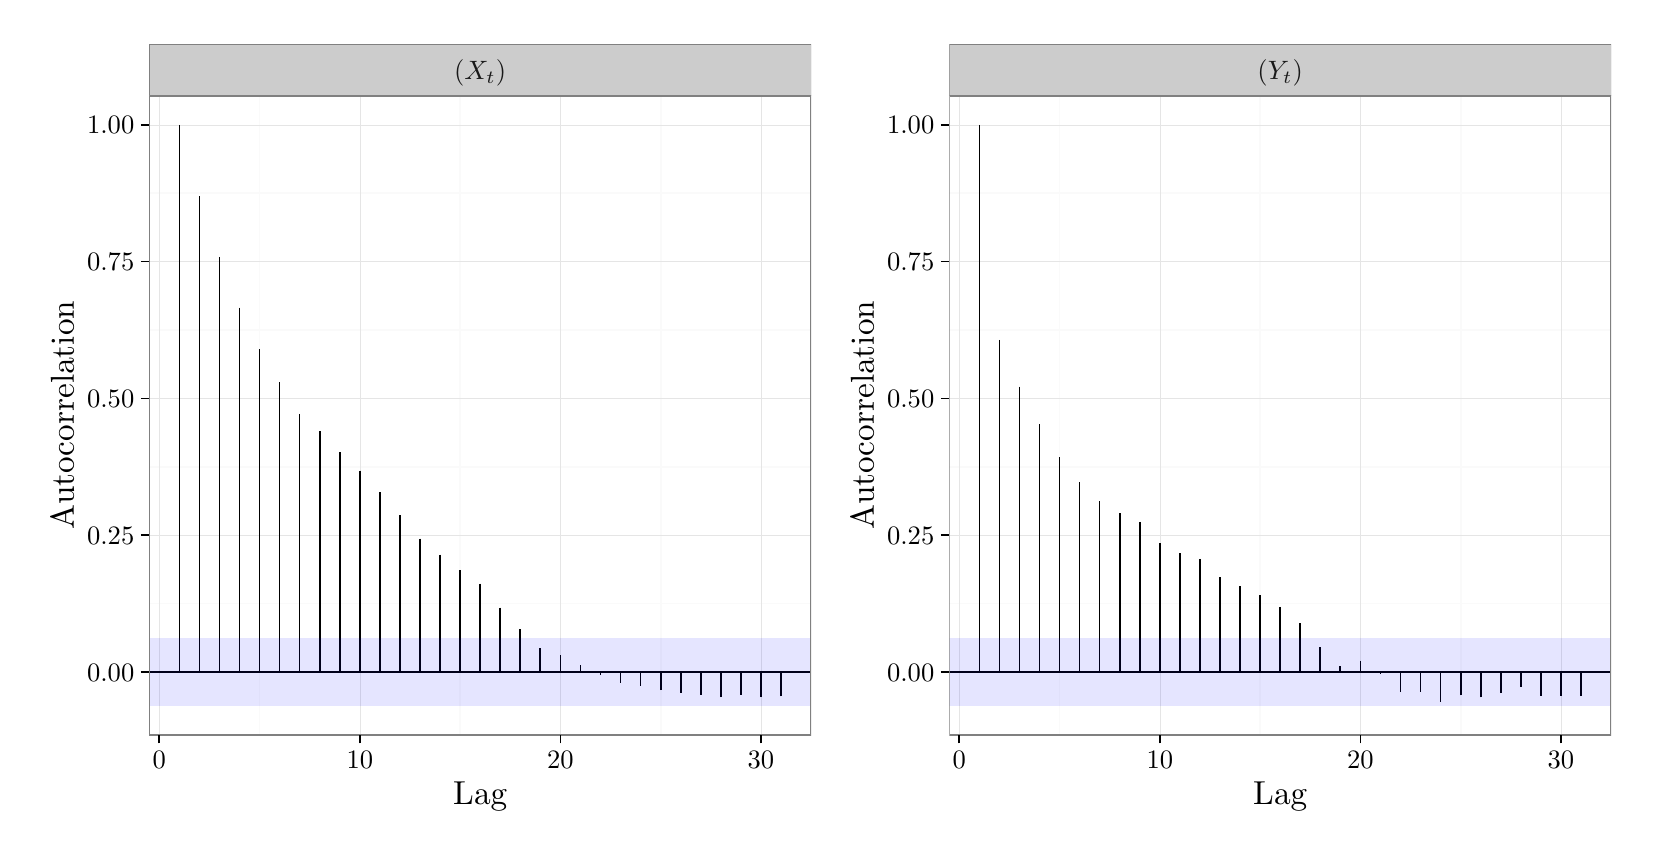
\begin{tikzpicture}[x=1pt,y=1pt]
\definecolor{fillColor}{RGB}{255,255,255}
\path[use as bounding box,fill=fillColor,fill opacity=0.00] (0,0) rectangle (578.16,289.08);
\begin{scope}
\path[clip] (  0.00,  0.00) rectangle (289.08,289.08);
\definecolor{drawColor}{RGB}{255,255,255}
\definecolor{fillColor}{RGB}{255,255,255}

\path[draw=drawColor,line width= 0.6pt,line join=round,line cap=round,fill=fillColor] (  0.00,  0.00) rectangle (289.08,289.08);
\end{scope}
\begin{scope}
\path[clip] ( 43.93, 33.48) rectangle (283.08,264.47);
\definecolor{fillColor}{RGB}{255,255,255}

\path[fill=fillColor] ( 43.93, 33.48) rectangle (283.08,264.47);
\definecolor{drawColor}{gray}{0.98}

\path[draw=drawColor,line width= 0.6pt,line join=round] ( 43.93, 80.95) --
	(283.08, 80.95);

\path[draw=drawColor,line width= 0.6pt,line join=round] ( 43.93,130.38) --
	(283.08,130.38);

\path[draw=drawColor,line width= 0.6pt,line join=round] ( 43.93,179.82) --
	(283.08,179.82);

\path[draw=drawColor,line width= 0.6pt,line join=round] ( 43.93,229.25) --
	(283.08,229.25);

\path[draw=drawColor,line width= 0.6pt,line join=round] ( 83.79, 33.48) --
	( 83.79,264.47);

\path[draw=drawColor,line width= 0.6pt,line join=round] (156.26, 33.48) --
	(156.26,264.47);

\path[draw=drawColor,line width= 0.6pt,line join=round] (228.73, 33.48) --
	(228.73,264.47);
\definecolor{drawColor}{gray}{0.90}

\path[draw=drawColor,line width= 0.2pt,line join=round] ( 43.93, 56.23) --
	(283.08, 56.23);

\path[draw=drawColor,line width= 0.2pt,line join=round] ( 43.93,105.67) --
	(283.08,105.67);

\path[draw=drawColor,line width= 0.2pt,line join=round] ( 43.93,155.10) --
	(283.08,155.10);

\path[draw=drawColor,line width= 0.2pt,line join=round] ( 43.93,204.53) --
	(283.08,204.53);

\path[draw=drawColor,line width= 0.2pt,line join=round] ( 43.93,253.97) --
	(283.08,253.97);

\path[draw=drawColor,line width= 0.2pt,line join=round] ( 47.55, 33.48) --
	( 47.55,264.47);

\path[draw=drawColor,line width= 0.2pt,line join=round] (120.02, 33.48) --
	(120.02,264.47);

\path[draw=drawColor,line width= 0.2pt,line join=round] (192.49, 33.48) --
	(192.49,264.47);

\path[draw=drawColor,line width= 0.2pt,line join=round] (264.96, 33.48) --
	(264.96,264.47);
\definecolor{drawColor}{RGB}{0,0,0}

\path[draw=drawColor,line width= 0.6pt,line join=round] ( 43.93, 56.23) -- (283.08, 56.23);

\path[draw=drawColor,line width= 0.6pt,line join=round] ( 54.80,253.97) -- ( 54.80, 56.23);

\path[draw=drawColor,line width= 0.6pt,line join=round] ( 62.04,228.14) -- ( 62.04, 56.23);

\path[draw=drawColor,line width= 0.6pt,line join=round] ( 69.29,206.28) -- ( 69.29, 56.23);

\path[draw=drawColor,line width= 0.6pt,line join=round] ( 76.54,187.96) -- ( 76.54, 56.23);

\path[draw=drawColor,line width= 0.6pt,line join=round] ( 83.79,172.80) -- ( 83.79, 56.23);

\path[draw=drawColor,line width= 0.6pt,line join=round] ( 91.03,160.99) -- ( 91.03, 56.23);

\path[draw=drawColor,line width= 0.6pt,line join=round] ( 98.28,149.55) -- ( 98.28, 56.23);

\path[draw=drawColor,line width= 0.6pt,line join=round] (105.53,143.25) -- (105.53, 56.23);

\path[draw=drawColor,line width= 0.6pt,line join=round] (112.77,135.71) -- (112.77, 56.23);

\path[draw=drawColor,line width= 0.6pt,line join=round] (120.02,128.99) -- (120.02, 56.23);

\path[draw=drawColor,line width= 0.6pt,line join=round] (127.27,121.27) -- (127.27, 56.23);

\path[draw=drawColor,line width= 0.6pt,line join=round] (134.52,112.92) -- (134.52, 56.23);

\path[draw=drawColor,line width= 0.6pt,line join=round] (141.76,104.41) -- (141.76, 56.23);

\path[draw=drawColor,line width= 0.6pt,line join=round] (149.01, 98.63) -- (149.01, 56.23);

\path[draw=drawColor,line width= 0.6pt,line join=round] (156.26, 93.00) -- (156.26, 56.23);

\path[draw=drawColor,line width= 0.6pt,line join=round] (163.50, 88.21) -- (163.50, 56.23);

\path[draw=drawColor,line width= 0.6pt,line join=round] (170.75, 79.47) -- (170.75, 56.23);

\path[draw=drawColor,line width= 0.6pt,line join=round] (178.00, 71.75) -- (178.00, 56.23);

\path[draw=drawColor,line width= 0.6pt,line join=round] (185.24, 64.89) -- (185.24, 56.23);

\path[draw=drawColor,line width= 0.6pt,line join=round] (192.49, 62.26) -- (192.49, 56.23);

\path[draw=drawColor,line width= 0.6pt,line join=round] (199.74, 58.75) -- (199.74, 56.23);

\path[draw=drawColor,line width= 0.6pt,line join=round] (206.99, 55.13) -- (206.99, 56.23);

\path[draw=drawColor,line width= 0.6pt,line join=round] (214.23, 52.29) -- (214.23, 56.23);

\path[draw=drawColor,line width= 0.6pt,line join=round] (221.48, 51.31) -- (221.48, 56.23);

\path[draw=drawColor,line width= 0.6pt,line join=round] (228.73, 49.73) -- (228.73, 56.23);

\path[draw=drawColor,line width= 0.6pt,line join=round] (235.97, 48.80) -- (235.97, 56.23);

\path[draw=drawColor,line width= 0.6pt,line join=round] (243.22, 48.00) -- (243.22, 56.23);

\path[draw=drawColor,line width= 0.6pt,line join=round] (250.47, 47.17) -- (250.47, 56.23);

\path[draw=drawColor,line width= 0.6pt,line join=round] (257.72, 47.96) -- (257.72, 56.23);

\path[draw=drawColor,line width= 0.6pt,line join=round] (264.96, 47.13) -- (264.96, 56.23);

\path[draw=drawColor,line width= 0.6pt,line join=round] (272.21, 47.42) -- (272.21, 56.23);
\definecolor{fillColor}{RGB}{0,0,255}

\path[fill=fillColor,fill opacity=0.10] ( 43.93, 43.98) rectangle (283.08, 68.49);
\definecolor{drawColor}{gray}{0.50}

\path[draw=drawColor,line width= 0.6pt,line join=round,line cap=round] ( 43.93, 33.48) rectangle (283.08,264.47);
\end{scope}
\begin{scope}
\path[clip] ( 43.93,264.47) rectangle (283.08,283.08);
\definecolor{drawColor}{gray}{0.50}
\definecolor{fillColor}{gray}{0.80}

\path[draw=drawColor,line width= 0.2pt,line join=round,line cap=round,fill=fillColor] ( 43.93,264.47) rectangle (283.08,283.08);
\definecolor{drawColor}{gray}{0.10}

\node[text=drawColor,anchor=base,inner sep=0pt, outer sep=0pt, scale=  0.96] at (163.50,270.47) {$(X_t)$};
\end{scope}
\begin{scope}
\path[clip] (  0.00,  0.00) rectangle (578.16,289.08);
\definecolor{drawColor}{RGB}{0,0,0}

\node[text=drawColor,anchor=base east,inner sep=0pt, outer sep=0pt, scale=  0.96] at ( 38.53, 52.93) {0.00};

\node[text=drawColor,anchor=base east,inner sep=0pt, outer sep=0pt, scale=  0.96] at ( 38.53,102.36) {0.25};

\node[text=drawColor,anchor=base east,inner sep=0pt, outer sep=0pt, scale=  0.96] at ( 38.53,151.79) {0.50};

\node[text=drawColor,anchor=base east,inner sep=0pt, outer sep=0pt, scale=  0.96] at ( 38.53,201.23) {0.75};

\node[text=drawColor,anchor=base east,inner sep=0pt, outer sep=0pt, scale=  0.96] at ( 38.53,250.66) {1.00};
\end{scope}
\begin{scope}
\path[clip] (  0.00,  0.00) rectangle (578.16,289.08);
\definecolor{drawColor}{RGB}{0,0,0}

\path[draw=drawColor,line width= 0.6pt,line join=round] ( 40.93, 56.23) --
	( 43.93, 56.23);

\path[draw=drawColor,line width= 0.6pt,line join=round] ( 40.93,105.67) --
	( 43.93,105.67);

\path[draw=drawColor,line width= 0.6pt,line join=round] ( 40.93,155.10) --
	( 43.93,155.10);

\path[draw=drawColor,line width= 0.6pt,line join=round] ( 40.93,204.53) --
	( 43.93,204.53);

\path[draw=drawColor,line width= 0.6pt,line join=round] ( 40.93,253.97) --
	( 43.93,253.97);
\end{scope}
\begin{scope}
\path[clip] (  0.00,  0.00) rectangle (578.16,289.08);
\definecolor{drawColor}{RGB}{0,0,0}

\path[draw=drawColor,line width= 0.6pt,line join=round] ( 47.55, 30.48) --
	( 47.55, 33.48);

\path[draw=drawColor,line width= 0.6pt,line join=round] (120.02, 30.48) --
	(120.02, 33.48);

\path[draw=drawColor,line width= 0.6pt,line join=round] (192.49, 30.48) --
	(192.49, 33.48);

\path[draw=drawColor,line width= 0.6pt,line join=round] (264.96, 30.48) --
	(264.96, 33.48);
\end{scope}
\begin{scope}
\path[clip] (  0.00,  0.00) rectangle (578.16,289.08);
\definecolor{drawColor}{RGB}{0,0,0}

\node[text=drawColor,anchor=base,inner sep=0pt, outer sep=0pt, scale=  0.96] at ( 47.55, 21.46) {0};

\node[text=drawColor,anchor=base,inner sep=0pt, outer sep=0pt, scale=  0.96] at (120.02, 21.46) {10};

\node[text=drawColor,anchor=base,inner sep=0pt, outer sep=0pt, scale=  0.96] at (192.49, 21.46) {20};

\node[text=drawColor,anchor=base,inner sep=0pt, outer sep=0pt, scale=  0.96] at (264.96, 21.46) {30};
\end{scope}
\begin{scope}
\path[clip] (  0.00,  0.00) rectangle (578.16,289.08);
\definecolor{drawColor}{RGB}{0,0,0}

\node[text=drawColor,anchor=base,inner sep=0pt, outer sep=0pt, scale=  1.20] at (163.50,  8.40) {Lag};
\end{scope}
\begin{scope}
\path[clip] (  0.00,  0.00) rectangle (578.16,289.08);
\definecolor{drawColor}{RGB}{0,0,0}

\node[text=drawColor,rotate= 90.00,anchor=base,inner sep=0pt, outer sep=0pt, scale=  1.20] at ( 16.66,148.97) {Autocorrelation};
\end{scope}
\begin{scope}
\path[clip] (289.08,  0.00) rectangle (578.16,289.08);
\definecolor{drawColor}{RGB}{255,255,255}
\definecolor{fillColor}{RGB}{255,255,255}

\path[draw=drawColor,line width= 0.6pt,line join=round,line cap=round,fill=fillColor] (289.08,  0.00) rectangle (578.16,289.08);
\end{scope}
\begin{scope}
\path[clip] (333.01, 33.48) rectangle (572.16,264.47);
\definecolor{fillColor}{RGB}{255,255,255}

\path[fill=fillColor] (333.01, 33.48) rectangle (572.16,264.47);
\definecolor{drawColor}{gray}{0.98}

\path[draw=drawColor,line width= 0.6pt,line join=round] (333.01, 80.95) --
	(572.16, 80.95);

\path[draw=drawColor,line width= 0.6pt,line join=round] (333.01,130.38) --
	(572.16,130.38);

\path[draw=drawColor,line width= 0.6pt,line join=round] (333.01,179.82) --
	(572.16,179.82);

\path[draw=drawColor,line width= 0.6pt,line join=round] (333.01,229.25) --
	(572.16,229.25);

\path[draw=drawColor,line width= 0.6pt,line join=round] (372.87, 33.48) --
	(372.87,264.47);

\path[draw=drawColor,line width= 0.6pt,line join=round] (445.34, 33.48) --
	(445.34,264.47);

\path[draw=drawColor,line width= 0.6pt,line join=round] (517.81, 33.48) --
	(517.81,264.47);
\definecolor{drawColor}{gray}{0.90}

\path[draw=drawColor,line width= 0.2pt,line join=round] (333.01, 56.23) --
	(572.16, 56.23);

\path[draw=drawColor,line width= 0.2pt,line join=round] (333.01,105.67) --
	(572.16,105.67);

\path[draw=drawColor,line width= 0.2pt,line join=round] (333.01,155.10) --
	(572.16,155.10);

\path[draw=drawColor,line width= 0.2pt,line join=round] (333.01,204.53) --
	(572.16,204.53);

\path[draw=drawColor,line width= 0.2pt,line join=round] (333.01,253.97) --
	(572.16,253.97);

\path[draw=drawColor,line width= 0.2pt,line join=round] (336.63, 33.48) --
	(336.63,264.47);

\path[draw=drawColor,line width= 0.2pt,line join=round] (409.10, 33.48) --
	(409.10,264.47);

\path[draw=drawColor,line width= 0.2pt,line join=round] (481.57, 33.48) --
	(481.57,264.47);

\path[draw=drawColor,line width= 0.2pt,line join=round] (554.04, 33.48) --
	(554.04,264.47);
\definecolor{drawColor}{RGB}{0,0,0}

\path[draw=drawColor,line width= 0.6pt,line join=round] (333.01, 56.23) -- (572.16, 56.23);

\path[draw=drawColor,line width= 0.6pt,line join=round] (343.88,253.97) -- (343.88, 56.23);

\path[draw=drawColor,line width= 0.6pt,line join=round] (351.12,176.29) -- (351.12, 56.23);

\path[draw=drawColor,line width= 0.6pt,line join=round] (358.37,159.41) -- (358.37, 56.23);

\path[draw=drawColor,line width= 0.6pt,line join=round] (365.62,145.71) -- (365.62, 56.23);

\path[draw=drawColor,line width= 0.6pt,line join=round] (372.87,133.88) -- (372.87, 56.23);

\path[draw=drawColor,line width= 0.6pt,line join=round] (380.11,124.76) -- (380.11, 56.23);

\path[draw=drawColor,line width= 0.6pt,line join=round] (387.36,117.99) -- (387.36, 56.23);

\path[draw=drawColor,line width= 0.6pt,line join=round] (394.61,113.64) -- (394.61, 56.23);

\path[draw=drawColor,line width= 0.6pt,line join=round] (401.85,110.50) -- (401.85, 56.23);

\path[draw=drawColor,line width= 0.6pt,line join=round] (409.10,102.79) -- (409.10, 56.23);

\path[draw=drawColor,line width= 0.6pt,line join=round] (416.35, 99.19) -- (416.35, 56.23);

\path[draw=drawColor,line width= 0.6pt,line join=round] (423.60, 97.14) -- (423.60, 56.23);

\path[draw=drawColor,line width= 0.6pt,line join=round] (430.84, 90.40) -- (430.84, 56.23);

\path[draw=drawColor,line width= 0.6pt,line join=round] (438.09, 87.15) -- (438.09, 56.23);

\path[draw=drawColor,line width= 0.6pt,line join=round] (445.34, 83.91) -- (445.34, 56.23);

\path[draw=drawColor,line width= 0.6pt,line join=round] (452.58, 79.74) -- (452.58, 56.23);

\path[draw=drawColor,line width= 0.6pt,line join=round] (459.83, 73.80) -- (459.83, 56.23);

\path[draw=drawColor,line width= 0.6pt,line join=round] (467.08, 65.16) -- (467.08, 56.23);

\path[draw=drawColor,line width= 0.6pt,line join=round] (474.32, 58.38) -- (474.32, 56.23);

\path[draw=drawColor,line width= 0.6pt,line join=round] (481.57, 60.27) -- (481.57, 56.23);

\path[draw=drawColor,line width= 0.6pt,line join=round] (488.82, 55.64) -- (488.82, 56.23);

\path[draw=drawColor,line width= 0.6pt,line join=round] (496.07, 48.94) -- (496.07, 56.23);

\path[draw=drawColor,line width= 0.6pt,line join=round] (503.31, 49.05) -- (503.31, 56.23);

\path[draw=drawColor,line width= 0.6pt,line join=round] (510.56, 45.50) -- (510.56, 56.23);

\path[draw=drawColor,line width= 0.6pt,line join=round] (517.81, 47.84) -- (517.81, 56.23);

\path[draw=drawColor,line width= 0.6pt,line join=round] (525.05, 47.08) -- (525.05, 56.23);

\path[draw=drawColor,line width= 0.6pt,line join=round] (532.30, 48.61) -- (532.30, 56.23);

\path[draw=drawColor,line width= 0.6pt,line join=round] (539.55, 50.87) -- (539.55, 56.23);

\path[draw=drawColor,line width= 0.6pt,line join=round] (546.80, 47.75) -- (546.80, 56.23);

\path[draw=drawColor,line width= 0.6pt,line join=round] (554.04, 47.66) -- (554.04, 56.23);

\path[draw=drawColor,line width= 0.6pt,line join=round] (561.29, 47.49) -- (561.29, 56.23);
\definecolor{fillColor}{RGB}{0,0,255}

\path[fill=fillColor,fill opacity=0.10] (333.01, 43.98) rectangle (572.16, 68.49);
\definecolor{drawColor}{gray}{0.50}

\path[draw=drawColor,line width= 0.6pt,line join=round,line cap=round] (333.01, 33.48) rectangle (572.16,264.47);
\end{scope}
\begin{scope}
\path[clip] (333.01,264.47) rectangle (572.16,283.08);
\definecolor{drawColor}{gray}{0.50}
\definecolor{fillColor}{gray}{0.80}

\path[draw=drawColor,line width= 0.2pt,line join=round,line cap=round,fill=fillColor] (333.01,264.47) rectangle (572.16,283.08);
\definecolor{drawColor}{gray}{0.10}

\node[text=drawColor,anchor=base,inner sep=0pt, outer sep=0pt, scale=  0.96] at (452.58,270.47) {$(Y_t)$};
\end{scope}
\begin{scope}
\path[clip] (  0.00,  0.00) rectangle (578.16,289.08);
\definecolor{drawColor}{RGB}{0,0,0}

\node[text=drawColor,anchor=base east,inner sep=0pt, outer sep=0pt, scale=  0.96] at (327.61, 52.93) {0.00};

\node[text=drawColor,anchor=base east,inner sep=0pt, outer sep=0pt, scale=  0.96] at (327.61,102.36) {0.25};

\node[text=drawColor,anchor=base east,inner sep=0pt, outer sep=0pt, scale=  0.96] at (327.61,151.79) {0.50};

\node[text=drawColor,anchor=base east,inner sep=0pt, outer sep=0pt, scale=  0.96] at (327.61,201.23) {0.75};

\node[text=drawColor,anchor=base east,inner sep=0pt, outer sep=0pt, scale=  0.96] at (327.61,250.66) {1.00};
\end{scope}
\begin{scope}
\path[clip] (  0.00,  0.00) rectangle (578.16,289.08);
\definecolor{drawColor}{RGB}{0,0,0}

\path[draw=drawColor,line width= 0.6pt,line join=round] (330.01, 56.23) --
	(333.01, 56.23);

\path[draw=drawColor,line width= 0.6pt,line join=round] (330.01,105.67) --
	(333.01,105.67);

\path[draw=drawColor,line width= 0.6pt,line join=round] (330.01,155.10) --
	(333.01,155.10);

\path[draw=drawColor,line width= 0.6pt,line join=round] (330.01,204.53) --
	(333.01,204.53);

\path[draw=drawColor,line width= 0.6pt,line join=round] (330.01,253.97) --
	(333.01,253.97);
\end{scope}
\begin{scope}
\path[clip] (  0.00,  0.00) rectangle (578.16,289.08);
\definecolor{drawColor}{RGB}{0,0,0}

\path[draw=drawColor,line width= 0.6pt,line join=round] (336.63, 30.48) --
	(336.63, 33.48);

\path[draw=drawColor,line width= 0.6pt,line join=round] (409.10, 30.48) --
	(409.10, 33.48);

\path[draw=drawColor,line width= 0.6pt,line join=round] (481.57, 30.48) --
	(481.57, 33.48);

\path[draw=drawColor,line width= 0.6pt,line join=round] (554.04, 30.48) --
	(554.04, 33.48);
\end{scope}
\begin{scope}
\path[clip] (  0.00,  0.00) rectangle (578.16,289.08);
\definecolor{drawColor}{RGB}{0,0,0}

\node[text=drawColor,anchor=base,inner sep=0pt, outer sep=0pt, scale=  0.96] at (336.63, 21.46) {0};

\node[text=drawColor,anchor=base,inner sep=0pt, outer sep=0pt, scale=  0.96] at (409.10, 21.46) {10};

\node[text=drawColor,anchor=base,inner sep=0pt, outer sep=0pt, scale=  0.96] at (481.57, 21.46) {20};

\node[text=drawColor,anchor=base,inner sep=0pt, outer sep=0pt, scale=  0.96] at (554.04, 21.46) {30};
\end{scope}
\begin{scope}
\path[clip] (  0.00,  0.00) rectangle (578.16,289.08);
\definecolor{drawColor}{RGB}{0,0,0}

\node[text=drawColor,anchor=base,inner sep=0pt, outer sep=0pt, scale=  1.20] at (452.58,  8.40) {Lag};
\end{scope}
\begin{scope}
\path[clip] (  0.00,  0.00) rectangle (578.16,289.08);
\definecolor{drawColor}{RGB}{0,0,0}

\node[text=drawColor,rotate= 90.00,anchor=base,inner sep=0pt, outer sep=0pt, scale=  1.20] at (305.74,148.97) {Autocorrelation};
\end{scope}
\end{tikzpicture}
